\documentclass[a4paper, 12pt]{article}

\usepackage{hyperref}
\usepackage[all]{hypcap}

\usepackage{mpsi}
\usepackage[utf8]{inputenc}
\usepackage{graphicx}
\usepackage{float}
\usepackage{amsmath}
\usepackage{setspace}

\usepackage[T1]{fontenc}
\usepackage{lmodern}

\usepackage{ragged2e}
\usepackage{pgfplots}
\usepackage{interval}
\usepackage{listings}

\usepackage{caption}
\captionsetup[figure]{format=plain,labelfont=bf,textfont=it,justification=centering}
\captionsetup[table]{format=plain,labelfont=bf,textfont=it,justification=centering}

\def\Titre{Détection d'un casino en ligne frauduleux}

\usepackage[top=2cm, bottom=2cm, left=2cm, right=2cm]{geometry}
\fancyhead[L]{Tom Dupont}
\fancyhead[R]{Centrale Lille}

\newtheoremstyle
{exo}
{}
{}
{\large}
{}
{\bfseries\scshape}
{}
{\newline}
{\thmname{#1} \thmnumber{#2} : \thmnote{{\bf(#3)}}}

\theoremstyle{exo}
\newtheorem{exo}{Exercice}

\begin{document}
\setstretch{2.25}
\pagestyle{fancy}
\justifying

\begin{center}
\textsc{\bfseries\huge \Titre}
\end{center}

\tableofcontents
\listoffigures
\listoftables

\newpage

\section{Mise en contexte}

On considère ici un jeu de données provenant d'un casino en ligne dans un pays qui a des restrictions sur les jeux d'argent en ligne (non spécifié). Le principe est le suivant : les joueurs peuvent parier des objets virtuels d'un jeu vidéo (des skins), ces skins ont une certaine valeur en euro (c'est donc comme s'ils parient de l'argent), et choisir un nombre entre 1 et $+\infty$. On tire alors une roulette fictive (la distribution des valeurs est inconnue) et il y a deux issues, si on est en dessous du nombre choisi on gagne sa mise mutlipliée par ce nombre et sinon on perd sa mise. On a un jeu de données de 55 575 parties, voici les 10 premières :

\begin{table}[ht]
\centering
\begin{tabular}{cccccccc}
    \hline
    & Joueurs & Argent & Pari & Victoire & Defaite & Gains & Moderateur \\ 
    \hline
2091103 & 144 & 283.57 & 14.30 & 125.46 & 0.25 & 408.78 &   0 \\ 
    2091104 & 134 & 279.30 & 1.14 & 5.81 & 177.04 & 108.07 &   0 \\ 
    2091105 & 139 & 282.87 & 3.91 & 125.01 & 5.96 & 401.92 &   0 \\ 
    2091106 & 139 & 271.44 & 1.15 & 6.90 & 181.85 & 96.49 &   0 \\ 
    2091107 & 142 & 304.88 & 1.00 & 0.00 & 304.88 & 0.00 &   0 \\ 
    2091108 & 161 & 463.81 & 2.46 & 118.96 & 15.45 & 567.32 &   0 \\ 
    2091109 & 157 & 342.79 & 1.45 & 36.50 & 119.43 & 259.86 &   0 \\ 
    2091110 & 160 & 302.06 & 2.73 & 93.70 & 25.94 & 369.82 &   0 \\ 
    2091111 & 155 & 1218.63 & 5.37 & 184.01 & 3.16 & 1399.48 &   0 \\ 
    2091112 & 129 & 236.01 & 2.09 & 64.04 & 12.02 & 288.03 &   0 \\ 
    \hline
\end{tabular}
\caption{Jeu de données}
\end{table}

\noindent La colonne joueurs représente le nombre de joueurs durant une partie, la colonne argent représente l'argent misé dans cette partie, la colonne pari représente le résultat de la roulette durant cette partie, la colonne victoire représente la quantité de bénéfice durant cette partie (en ayant retiré la mise) , la colonne défaite représente la quantité d'argent perdu durant cette partie, la colonne gains représente la quantité d'argent gagné durant cette partie (sans avoir retiré la mise), la colonne modérateur représente s'il y a ou non un modérateur durant cette partie.\\

\newpage

Tout d'abord, on peut tracer la distribution des valeurs de la colonne pari :

\begin{figure}[H]
\centering
\includegraphics[width=\textwidth]{figures/densité_paris.png}
\caption{Distribution des valeurs de la colonne pari}
\end{figure}

\noindent A première vue, on peut voir que la distribution est régulière, on peut donc penser naïvement que le casino n'est pas truqué. Cependant, nous allons voir au travers différentes analyses que c'est tout à fait l'inverse.

\newpage

\section{Analyse de données}
\subsection{Analyse en composantes principales}

Tout d'abord, nous avons réalisé une analyse en composantes principales. Voici en premier lieu le graphe d'inertie des valeurs propres :

\begin{figure}[H]
\centering
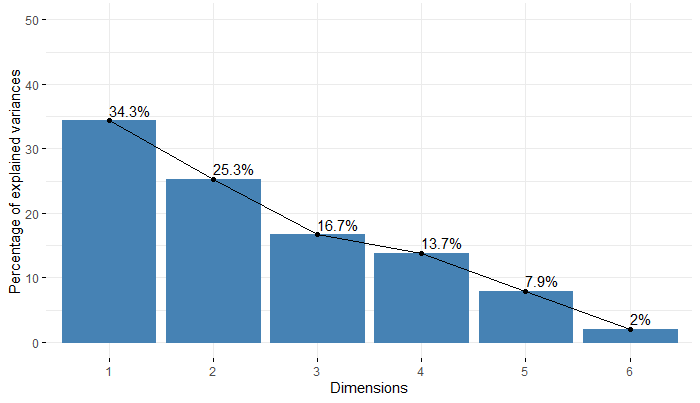
\includegraphics[width=0.8\textwidth]{figures/Valeurs_propres.png}
\caption{Graphe d'inertie des valeurs propres}
\end{figure}

\noindent On peut voir que les deux premières composantes principales représentent à elles seules 60\% de l'inertie totale, on va donc se contenter de les étudier. Voici à présent la carte factorielle couplé du cercle des corrélations :

\begin{figure}[H]
\centering
    \begin{minipage}{0.58\textwidth}
        \centering
        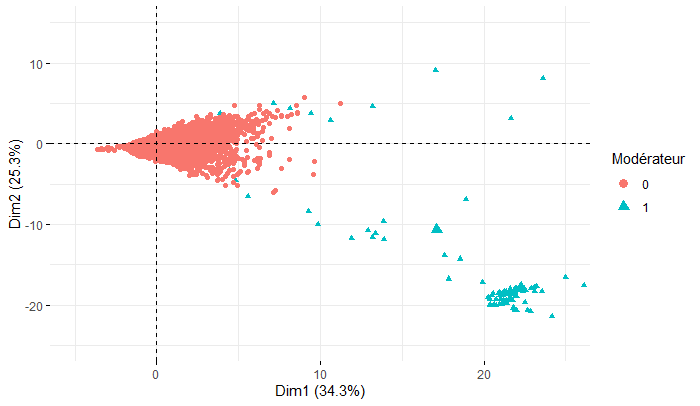
\includegraphics[width=\textwidth]{figures/Individus.png}
        \caption{Carte factorielle}
    \end{minipage}
    \begin{minipage}{0.41\textwidth}
        \centering
        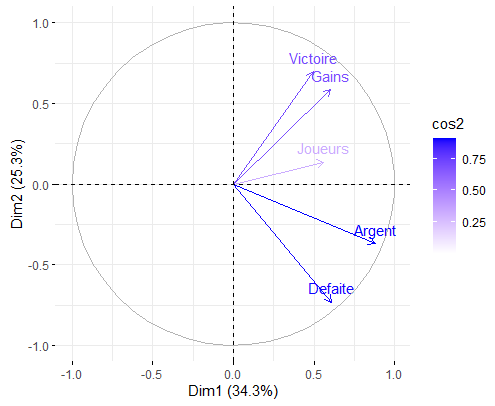
\includegraphics[width=\textwidth]{figures/Cercle.png}
        \caption{Cercle des corrélations}
    \end{minipage}
\end{figure}

\noindent Lorsqu'on représente les parties en fonction de si il y a un modérateur ou non, on remarque que les parties avec modérateur sont très proches les unes des autres, ce qui signifie que les parties avec modérateur sont très similaires entre elles. On remarque également que les parties avec modérateurs sont très corrélées aux colonnes argent et défaite, ce qui signifie que les parties avec modérateur sont très corrélées à la mise et à la perte. On peut donc penser que les parties avec modérateur sont des parties où les joueurs misent beaucoup d'argent et perdent beaucoup d'argent. Sûrement que les modérateurs misent beaucoup d'argent en étant sûrs de gagner et avec un score de roulette très faible ce qui expliquerait la corrélation avec la colonne défaite.

\subsection{Analyse en clusters}

Lorsqu'on réalise une analyse en clusters sur les deux premières composantes principales, on obtient la figure suivante :

\begin{figure}[H]
\centering
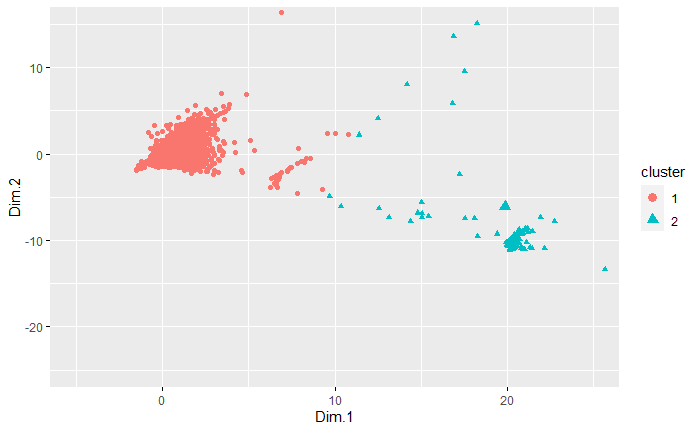
\includegraphics[width=\textwidth]{figures/Cluster.png}
\caption{Analyse en clusters}
\end{figure}

\noindent On remarque que les deux clusters trouvés coïncident avec la présence ou non d'un modérateur. On peut donc penser que les parties avec modérateur sont très différentes des parties sans modérateur. 

\subsection{Analyse discriminante}

A présent, faisons une analyse discriminante sur le fait qu'il y ait ou non un modérateur. Voici le tableau des moyennes selon la présence d'un modérateur :

\begin{table}[ht]
\centering
\begin{tabular}{ccccccc}
    \hline
    & Joueurs & Argent & Pari & Victoire & Defaite & Gains \\ 
    \hline
0 & 123.01 & 277.69 & 12.05 & 65.80 & 72.76 & 271.07 \\ 
    1 & 131.90 & 3208.31 & 3.18 & 402.30 & 2692.85 & 784.45 \\ 
    \hline
\end{tabular}
\caption{Moyennes selon la présence d'un modérateur}
\end{table}

\noindent On remarque que les moyennes sont très différentes selon la présence d'un modérateur. On confirme aussi nos suppositions quant à la partie 2.1, les parties avec modérateur sont des parties où les joueurs misent beaucoup d'argent et perdent beaucoup d'argent. On remarque également que les moyennes de la colonne pari sont très différentes, elle est beaucoup plus basse dans le cas d'une partie avec modérateur ce qui signifie que les modérateurs influencent la roulette pour qu'elle soit plus faible en misant peu et en faisant perdre beaucoup d'argent aux joueurs.

\newpage

On peut aussi visualiser le résultat de l'analyse discriminante :

\begin{figure}[H]
\centering
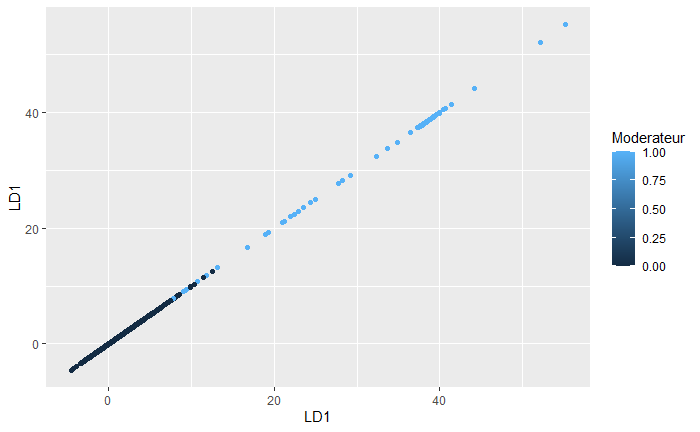
\includegraphics[width=0.8\textwidth]{figures/Predict.png}
\caption{Résultat de l'analyse discriminante}
\end{figure}

\noindent On remarque encore une fois que les deux groupes sont très bien séparés, ce qui confirme nos suppositions.

\subsection{Test du $\chi^2$}

À présent on peut finalement réaliser un test du $\chi^2$ entre la valeur de la roulette et la présence d'un modérateur. On obtient alors un $\chi^2$ de 666880 et une p-value de $2.2 \times 10^{-16}$, on rejette donc l'hypothèse nulle et on peut affirmer que la valeur de la roulette est dépendante de la présence d'un modérateur. On peut donc affirmer que le casino est truqué.  

\subsection{ANOVA}

En effectuant une ANOVA sur la valeur de la roulette en fonction de la présence d'un modérateur, on obtient la table suivante :

\begin{table}[H]
    \centering
    \begin{tabular}{lccccc}
      \hline
     & Df & Sum Sq & Mean Sq & F value & Pr($>$F) \\ 
      \hline
    Moderateur  & 1 & 10911.00 & 10911.00 & 0.19 & 0.6641 \\ 
      Residuals   & 55573 & 3214320632.19 & 57839.61 &  &  \\ 
       \hline
    \end{tabular}
    \caption{ANOVA avec toutes les données}
\end{table}

Les résultats de l'ANOVA montrent une valeur F de 0.189 et une p-value de 0.664. La valeur F est relativement faible, ce qui suggère que la variabilité entre les groupes n'est pas particulièrement grande par rapport à la variabilité à l'intérieur des groupes. Plus important encore, la p-value, qui est bien au-dessus du seuil conventionnel de 0.05, indique qu'il n'y a pas de différence statistiquement significative entre les montants moyens des paris dans les situations avec et sans modérateur. Ce qui contredit les résultats de l'analyse discriminante et du test du $\chi^2$, il faut noter que ces résultats ne sont pas complètement contradictoires, car la taille des deux échantillons est très différente.\\
On va alors recommencer l'ANOVA mais en choisissant aléatoirement 139 valeurs de la roulette sans modérateurs pour avoir un échantillon de même taille que celui avec modérateurs. On obtient alors la table suivante :

\begin{table}[H]
    \centering
    \begin{tabular}{lccccc}
      \hline
     & Df & Sum Sq & Mean Sq & F value & Pr($>$F) \\ 
      \hline
    Moderateur  & 1 & 477.60 & 477.60 & 3.93 & $0.0483^*$ \\ 
      Residuals   & 276 & 33503.04 & 121.39 &  &  \\ 
       \hline
    \end{tabular}
    \caption{ANOVA avec des données réduites}
\end{table}

On obtient alors une valeur F de 3.93 et une p-value de 0.0483 significative, on peut donc affirmer que la valeur de la roulette est dépendante de la présence d'un modérateur.

\subsection{Analyse factorielle des correspondances}

A présent nous allons réaliser une analyse factorielle des correspondances sur la présence d'un modérateur. Voici le graphe d'inertie des valeurs propres :

\begin{figure}[H]
\centering
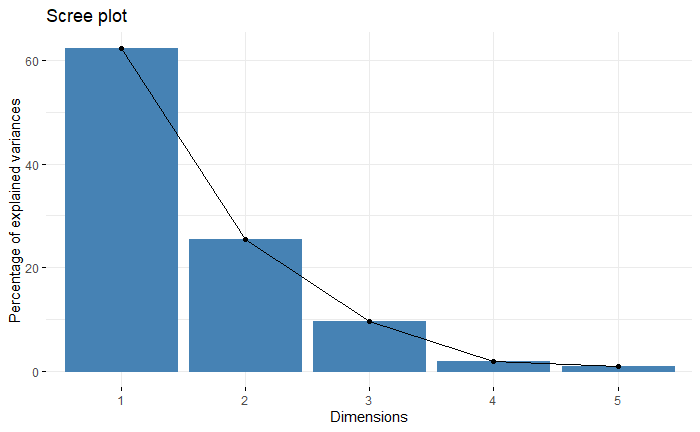
\includegraphics[width=0.8\textwidth]{figures/afc_vp.png}
\caption{Graphe d'inertie des valeurs propres}
\end{figure}

\noindent On peut voir que les deux premières composantes principales représentent à elles seules 87\% de l'inertie totale, on va donc se contenter de les étudier. Voici à présent la carte factorielle où les point sont différenciés selon la présence d'un modérateur et le graphe des colonnes :

\begin{figure}[H]
\centering
    \begin{minipage}{0.49\textwidth}
        \centering
        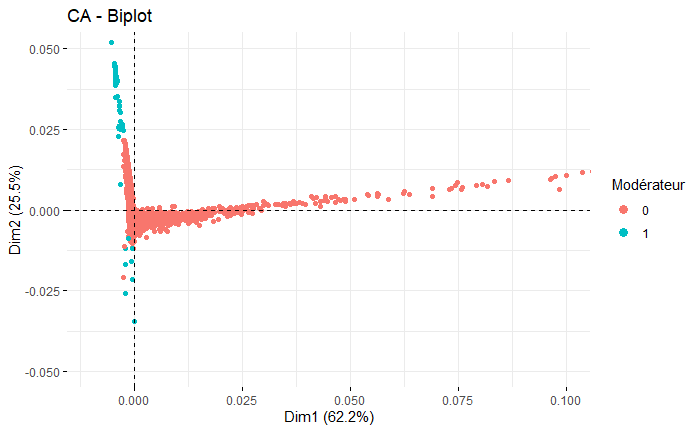
\includegraphics[width=\textwidth]{figures/biplot.png}
        \caption{Carte factorielle}
    \end{minipage}
    \begin{minipage}{0.49\textwidth}
        \centering
        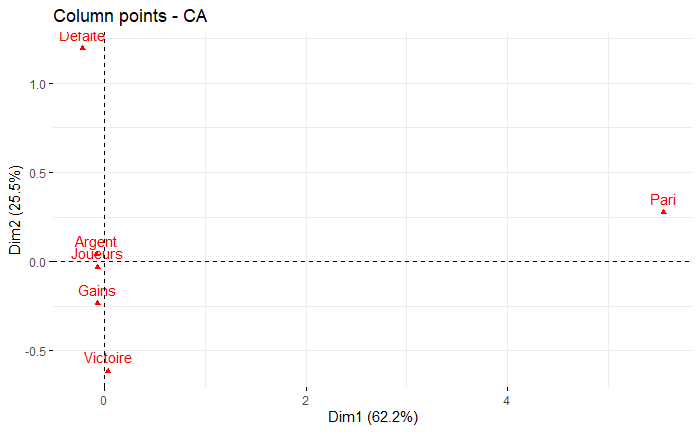
\includegraphics[width=\textwidth]{figures/afc_point.png}
        \caption{Graphe des colonnes}
    \end{minipage}
\end{figure}

Encore une fois, on remarque que les parties avec modérateur sont très corrélées avec la colonne défaite mais très peu avec la colonne Pari, ce qui est cohérent avec les différentes analyses faites précédemment.

\begin{lstlisting}[label={lst:afccode}]
    # Votre code R ici
    library(FactoMineR)
    res.ca <- CA(casino)
    fviz_ca_biplot(res.ca, geom = "point")
\caption{test}
\end{lstlisting}

\newpage

\section{Conclusion}

Pour résumer, à travers toutes ces différentes analyses de données, on a pu démontrer que le casino est truqué. En effet, on a pu voir que les parties avec modérateur sont très différentes des parties sans modérateur, les joueurs perdent beaucoup plus d'argent lors de parties avec modérateurs car la valeur de la roulette est artificiellement plus faible. Paradoxalement les joueurs misent beaucoup plus d'argent lors de parties avec modérateurs, ce qui signifie que les modérateurs misent beaucoup d'argent en étant sûrs de gagner.  

\end{document}